\section{Supporting figures}
\label{app:secondary}
The visibility-conditioned oracle of Section~\ref{sec:conventions} and the two secondary axes of
Section~\ref{sec:controls} are stated numerically in the main text; their figures are placed here.

\begin{figure}[htbp]
\centering
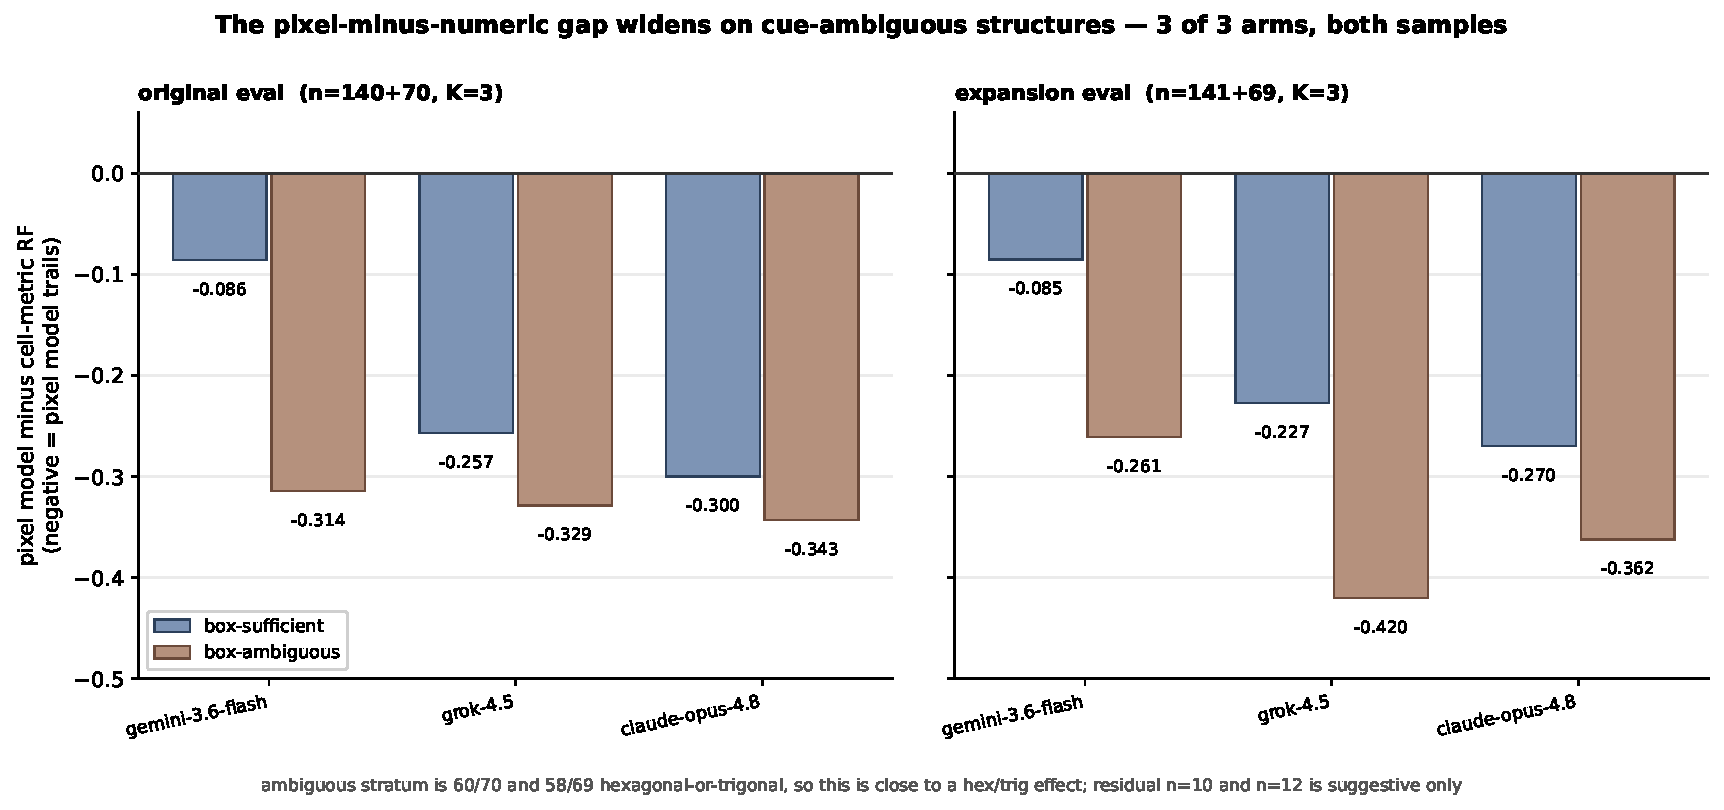
\includegraphics[width=0.8\linewidth]{figures/cuesuff.pdf}
\caption{Pixel accuracy minus a cell-metric random forest on the same structures, by cue-sufficiency
stratum, three frontier models, both evaluation samples ($K=3$). Negative means the pixel model trails the
numeric reader. Stratum composition is annotated on the panels; see Section~\ref{sec:controls}.}
\label{fig:cuesuff}
\end{figure}

\begin{figure}[htbp]
\centering
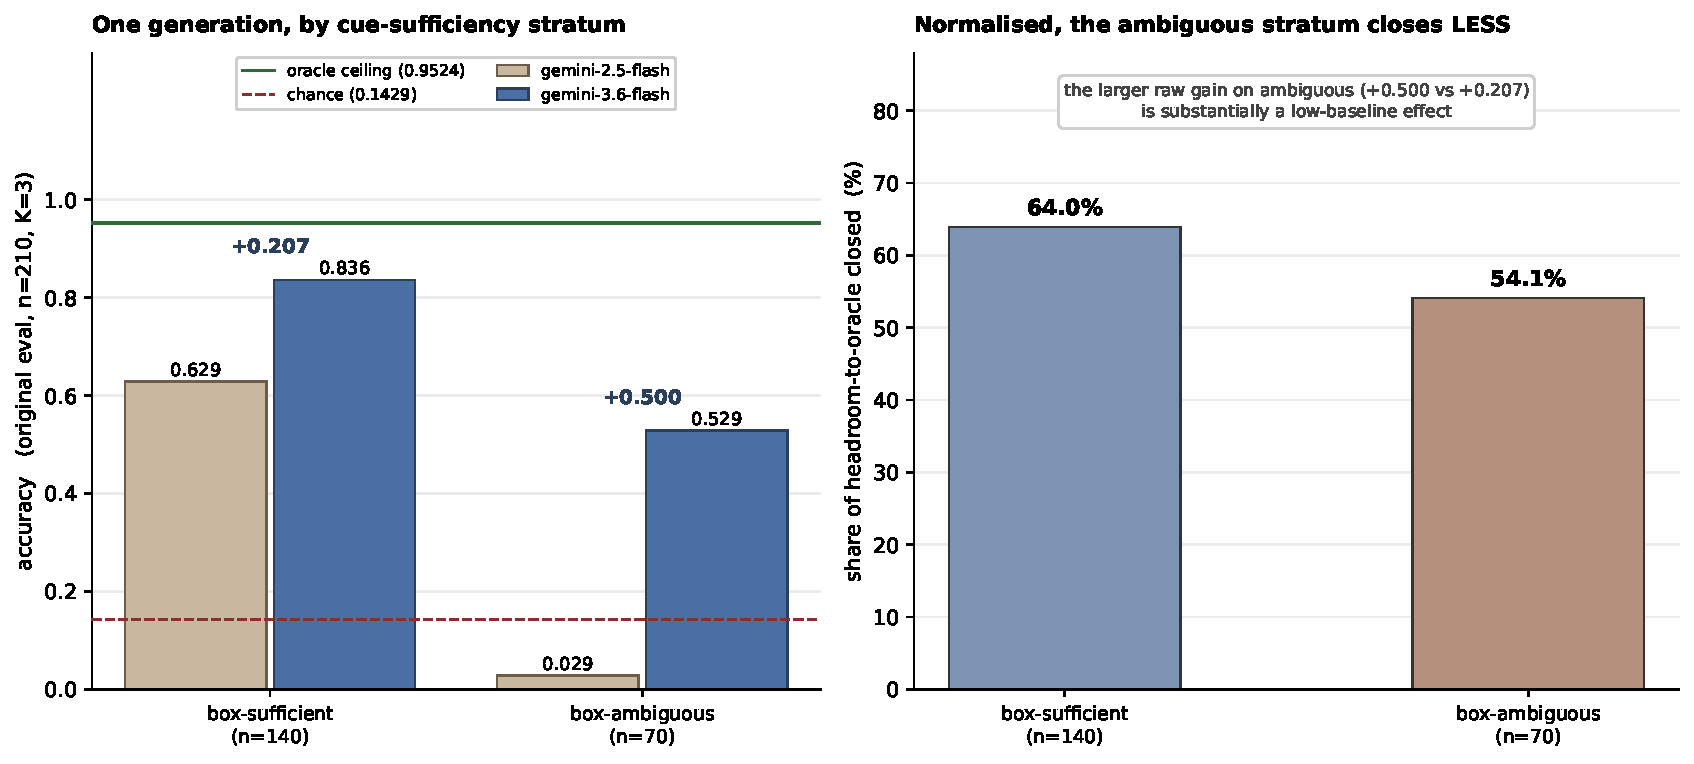
\includegraphics[width=0.8\linewidth]{figures/generational.pdf}
\caption{One generation of model progress, original sample, $n=210$, $K=3$. Left: raw accuracy by
cue-sufficiency stratum, with the oracle ceiling and seven-way chance drawn. Right: the same gains
normalised by headroom to the oracle.}
\label{fig:generational}
\end{figure}

\begin{figure}[htbp]
\centering
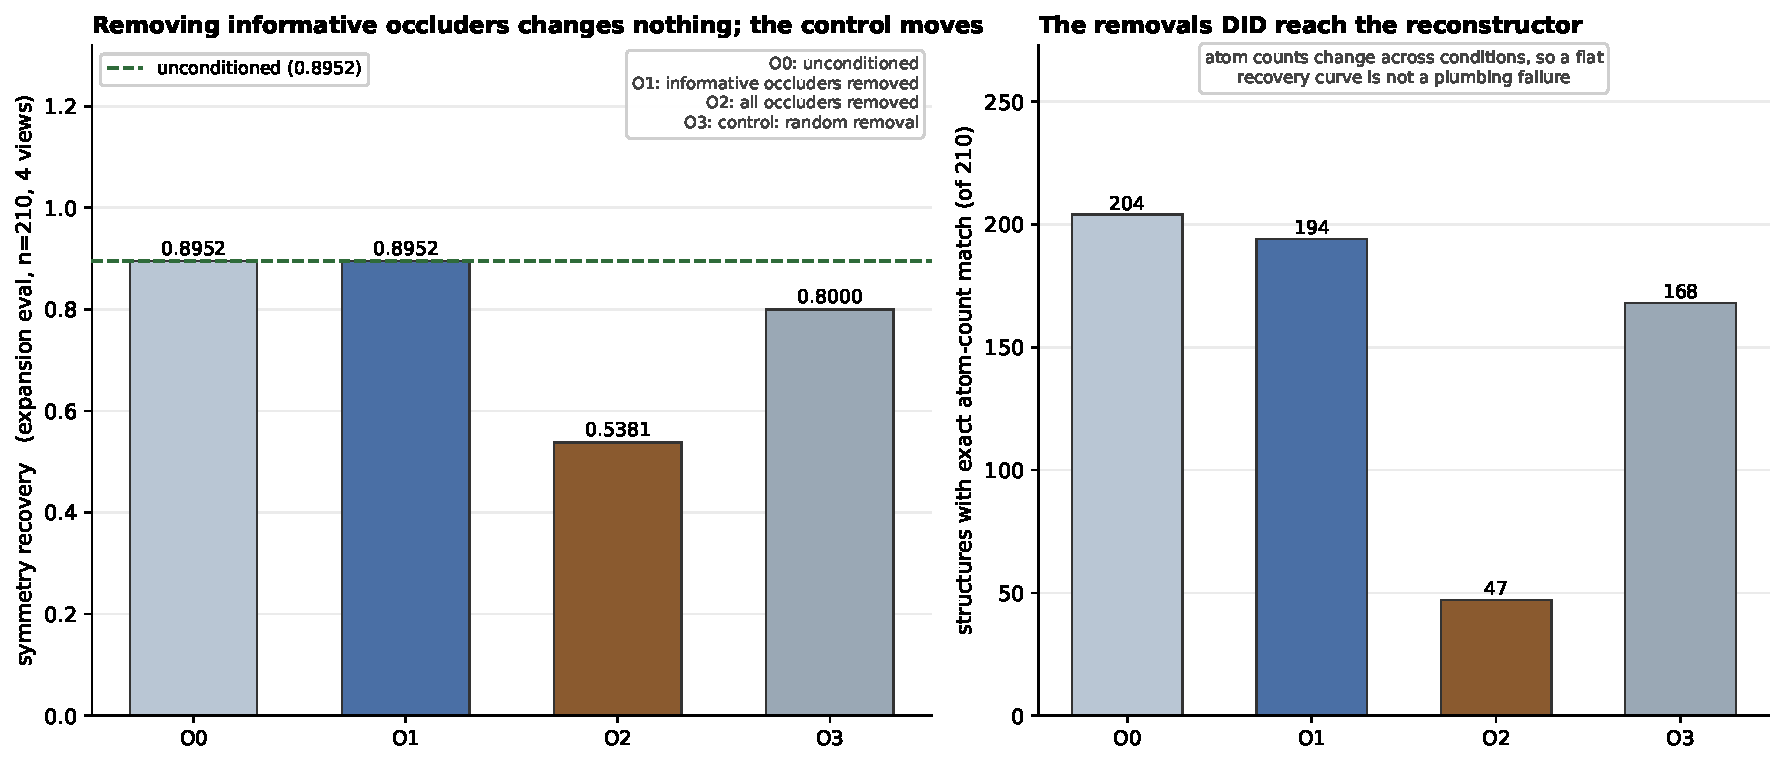
\includegraphics[width=0.8\linewidth]{figures/conditions.pdf}
\caption{Visibility-conditioned oracle: recovery when informative occlusion is removed from the oracle's
input, when redundant occlusion only is removed (pre-registered control), and unconditioned, on both
evaluation samples.}
\label{fig:conditions}
\end{figure}
